\chapter{Machine Learning Models Explored}

This section describes the process of choosing the architectural and regularization hyperparamers for each model. The section also describes the datasets used to train the models 

The simplest model explored is the DNN. Because of the high dimension of the input data, feature extraction methods will be implemented and compared. These methods include PCA, a DAE, and a CAE. 

The other general architecture that will be explored is a 1D CNN. 

\subsection{Training Templates Overview}

The datasets used to train the models are created using templates of simulated gamma-ray spectra without Poisson noise. A one-dimensional particle transport code developed at Sandia National Laboratory, GADRAS-DRF (Gamma Detector Response and Analysis Software - Detector Response Function), was used to generate these templates. This simulation code can be used to model physical conditions that affect spectra. For example, spectra change due to changes in measurement geometry. These changes include source-to-detector distance and the distance of both the detector and source from objects in an environment. To demonstrate this effect, $^{60}$Co spectra were simulated at various source-to-detector distances, Figure \ref{fig:sim_spectra_distance_comparison}, and heights off ground, Figure \ref{fig:sim_spectra_height_comparison}. These parameters change the the shape of the Compton continuum, the peak-to-total ratio, and the magnitude of the backscatter peak. Another parameter that changes the spectrum is the Gaussian energy broadening of the photopeaks. Due to manufacturing differences, each detector has a different amount of energy broadening. Examples of $^{60}$Co spectra with different broadening parameters are shown in Figure \ref{fig:sim_spectra_FWHM_comparison}.


\begin{figure}[H]
\centering
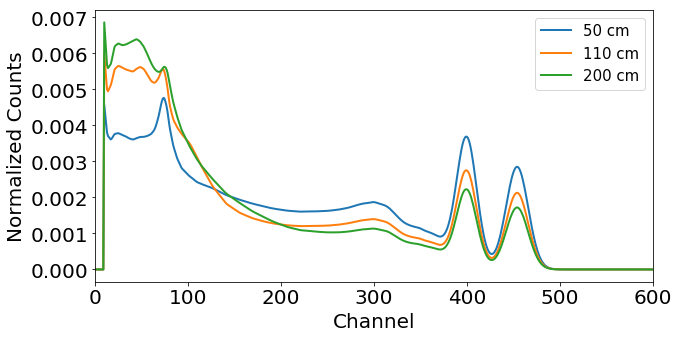
\includegraphics[width=0.75\linewidth]{images/sim_spectra_distance_comparison}
\caption{Comparison of a $^{60}$Co spectrum simulated at various source-detector distances.}
\label{fig:sim_spectra_distance_comparison}
\end{figure}

\begin{figure}[H]
\centering
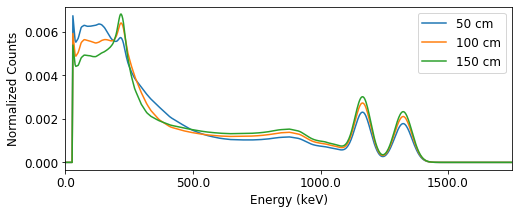
\includegraphics[width=0.75\linewidth]{images/sim_spectra_height_comparison}
\caption{Comparison of a $^{60}$Co spectrum simulated at various source-detector heights off the ground.}
\label{fig:sim_spectra_height_comparison}
\end{figure}


\begin{figure}[H]
\centering
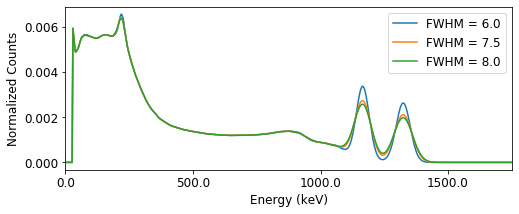
\includegraphics[width=0.75\linewidth]{images/sim_spectra_FWHM_comparison}
\caption{Comparison of a $^{60}$Co spectrum simulated with various FWHM parameters.}
\label{fig:sim_spectra_FWHM_comparison}
\end{figure}




% To incorporate these changes, templates simulated at different distances are included in the dataset. These distances start at 30cm, which is the distance at which a 1 uCi source will have an activity of about 400 cps on a 2 inch diameter detector. This is about twice the expected activity of background. 

% Changes in calibration due to temperature shifts are also considered. Due to the relatively large magnitude in calibration shifts due to temperature shifts from -5 C to 40 C \cite{CASANOVAS2012588}, it is expected incorporating these additions will also make the algorithm robust against calibration.

The template parameters used in this study are shown in Table \ref{table:all_fixed_simulation_parameters}. These parameters are based on handheld RIID scenarios. The source-detector height off ground are sampled between average shin and arm heights. The source-detector distance range corresponds to expected standoff distances. The areal density of each material corresponds to a 20$\%$, 40$\%$, 60$\%$, and 80$\%$ attenuation of a 200 keV photon. The photon energy was chosen because it is near the 186 keV energy of the most important $^{235}$U photopeak. A set of unshielded templates is also included. The FWHM range was chosen based on reported FWHM values for a NaI(Tl) detector (see section \ref{subsection_energy_resolution}). Background locations were chosen based on their geographic and geologic differences.

In addition to the parameters simulated by GADRAS-DRF, parameters are included to perform data augmentation. These parameters are shown in Table \ref{table:all_variable_simulation_parameters}.

\begin{table}[H]
\centering
\caption{Fixed GADRAS-DRF simulation parameters.}
\begin{tabular}{cc}
Parameter & Values \\ \hline
\begin{tabular}[c]{@{}c@{}}source-detector height \\ off ground {[}cm{]}\end{tabular} & 50.0, 75.0, 100.0, 125.0, 150.0 \\ 
\begin{tabular}[c]{@{}c@{}}source-detector\\ distance {[}cm{]}\end{tabular} & \multicolumn{1}{c}{50.0, 112.5, 175.0, 237.5, 300.0} \\ 
\begin{tabular}[c]{@{}c@{}}Areal density of \\ solid aluminum {[}g/cm\textasciicircum{}2{]}\end{tabular} & 1.82, 4.18, 7.49, 13.16 \\ 
\begin{tabular}[c]{@{}c@{}}Areal density of\\  solid iron {[}g/cm\textasciicircum{}2{]}\end{tabular} & 1.53, 3.5, 6.28, 11.02 \\ 
\begin{tabular}[c]{@{}c@{}}Areal density of \\ solid lead {[}g/cm\textasciicircum{}2{]}\end{tabular} & 0.22, 0.51, 0.92, 1.61 \\ 
\begin{tabular}[c]{@{}c@{}}FWHM at\\  662 keV {[}\%{]}\end{tabular} & \multicolumn{1}{c}{6.0, 6.5, 7.0, 7.5, 8.0, 8.5, 9.0} \\ 
\begin{tabular}[c]{@{}c@{}}Background\\ Location \end{tabular} & \begin{tabular}[c]{@{}c@{}}Albuquerque, Atlanta, Austin,\\ Chicago , Knoxville , Miami\end{tabular}
\end{tabular}
\label{table:all_fixed_simulation_parameters}
\end{table}

\begin{table}[H]
\centering
\caption{Default data augmentation parameters.}
\begin{tabular}{c}
Parameter \\ \hline
integration time \\ 
background counts per second \\ 
Signal to Background ratio \\ 
Calibration - Offset \\ 
Calibration - Gain \\ 
\end{tabular}
\label{table:all_variable_simulation_parameters}
\end{table}

% \begin{table}[H]
% \centering
% \caption{Default data augmentation parameters.}
% \begin{tabular}{ccc}
% Parameter & Values & Sampling \\ \hline
% integration time & 60 - 600 & uniform \\ 
% background counts per second & 200 & Poisson \\ 
% Signal to Background ratio & 0.5 - 2 & uniform \\ 
% 0th order calibration & 0 - 10 & uniform \\ 
% 1st order calibration & 0.83 - 1.16 & uniform \\ 
% \end{tabular}
% \label{table:all_variable_simulation_parameters}
% \end{table}


\section{Datasets Used for the Hyperparameter Search}

To investigate which parameters affect generalization performance, networks were trained using a simple and complete set of template simulation parameters. The parameters used for the simplified dataset are shown in Table \ref{table:hyperparameter_dataset_easy_parameters} and parameters used for the complete dataset are shown in Table \ref{table:hyperparameter_dataset_full_parameters}. Both datasets are comprised of the following isotopes from ANSI N42-34-2006 \cite{ANSI}: $^{241}$Am, $^{133}$Ba, $^{57}$Co, $^{60}$Co, $^{51}$Cr, $^{137}$Cs, $^{152}$Eu, $^{67}$Ga, $^{123}$I, $^{125}$I, $^{131}$I, $^{111}$In, $^{192}$Ir, $^{177m}$Lu, $^{99}$Mo, $^{237}$Np, $^{103}$Pd, $^{239}$Pu, $^{240}$Pu, $^{226}$Ra, $^{75}$Se, $^{153}$Sm, $^{99m}$Tc, $^{201}$Tl, $^{204}$Tl, $^{233}$U, $^{235}$U, $^{238}$U, and $^{133}$Xe.

Because datasets of different complexity often need different architectures and hyperparameters \cite{Bergstra2012}, independent hyperparameter searches were conducted for both datasets. For each dataset, a total of 100 spectra were simulated for each isotope. Each spectrum was simulated with parameters randomly sampled from the simple or complete parameter set.

\begin{table}[H]
\centering
\caption{Range of parameters used for the simple dataset.}
\label{table:hyperparameter_dataset_easy_parameters}
\begin{tabular}{ccc}
% \cline{2-3}
 & Hyperparameter Range & Sampling \\ \hline
\multicolumn{1}{c}{Source-Detector Distance {[}cm{]}} & 175.0 & N/A \\ 
\multicolumn{1}{c}{Source-Detector Height {[}cm{]}} & 100.0 & N/A \\ 
\multicolumn{1}{c}{FWHM 662 keV {[}s{]}} & 7.5 & N/A \\ 
\multicolumn{1}{c}{\begin{tabular}[c]{@{}c@{}}Shielding\\ (Percent 662 keV Attenuated)\end{tabular}} & 0\%, 20\% & Uniform \\ 
\multicolumn{1}{c}{Integration Time {[}s{]}} & 60 - 600 & Log-Uniform \\ 
\multicolumn{1}{c}{Calibration - Offset (channels)} & 0 - 10 & Uniform \\ 
\multicolumn{1}{c}{Calibration - Gain} & 0.9 - 1.1 & Uniform \\ 
\multicolumn{1}{c}{Signal to Background Ratio} & 0.5 - 2.0 & Uniform \\ 
\multicolumn{1}{c}{Background Counts Per Second} & 200 & Poisson \\ 
\end{tabular}
\end{table}


\begin{table}[H]
\centering
\caption{Range of parameters used for the complete dataset.}
\label{table:hyperparameter_dataset_full_parameters}
\begin{tabular}{ccc}
% \cline{2-3}
 & Hyperparameter Range & Sampling \\ \hline
\multicolumn{1}{c}{Source-Detector Distance {[}cm{]}} & 50.5, 175.0, 300 & Uniform \\ 
\multicolumn{1}{c}{Source-Detector Height {[}cm{]}} & 50, 100.0, 150 & Uniform \\ 
\multicolumn{1}{c}{FWHM 662 keV {[}s{]}} & 7.0, 7.5, 8.0 & Uniform \\ 
\multicolumn{1}{c}{\begin{tabular}[c]{@{}c@{}}Shielding\\ (Percent 662 keV Attenuated)\end{tabular}} & 0\%, 20\%, 40\%, 60\% & Uniform \\ 
\multicolumn{1}{c}{Integration Time {[}s{]}} & 10 - 3600 & Log-Uniform \\ 
\multicolumn{1}{c}{Calibration - Offset (channels)} & 0 - 10 & Uniform \\ 
\multicolumn{1}{c}{Calibration - Gain} & 0.8 - 1.2 & Uniform \\ 
\multicolumn{1}{c}{Signal to Background Ratio} & 0.1 - 3.0 & Uniform \\ 
\multicolumn{1}{c}{Background Counts Per Second} & 200 & Poisson \\ 
\end{tabular}
\end{table}


\section{Hyperparameter Search Results}

To determine an optimum combination of hyperparameters, a random hyperparameter search over hyperparameters was performed. For each network and both datasets, the average testing set error from 5-fold cross validation was recorded. An early stopping patience of 20 epochs was used to train 128 models. The maximum number of epochs was set to 200. The results of the hyperparameter searches are shown using random efficiency curves and by comparing parameter values versus average F1 scores in the testing set. Random efficiency curves indicate the quality of the hyperparameter search space and allows for reproducibility. Analyzing how the parameter values change the F1 score gives us an idea of which parameters are important. Hyperparameter bounds are based on previous published and unpublished experiments as well as recommendations from literature \cite{Bengio2018}.

% A sharper efficiency curve shows that many hyperparameter combinations perform well, whereas 

% The shape of this curve indicates the frequency of good models under random search, and quantifies the relative volumes (in search space) of the various levels of performance - Bergstra2012a


% These also allow for researchers who want to fit models to this dataset to have a performance benchmark. If you wanted to compare random hyperparameter search to more intelligent methods, you could compare using this.

\subsection{Dense Architecture}

Architecture and training hyperparamters are shown in Table \ref{table:hyperparameter_dataset_parameters_DNN}. Note, the number of nodes in each layers was made to decrease for each subsequent layer. The input scaling is read left-to-right. For example, the sqrt-max scaling would first take the square root of the each channel in the spectrum and then normalized the spectrum by its maximum value. The L1 norm normalizes a spectrum by its L1 norm. The log1p function is the base 10 logarithm of the input plus one.

\begin{table}[H]
\centering
\caption{Range of hyperparameters explored for the DNN.}
\label{table:hyperparameter_dataset_parameters_DNN}
\begin{tabular}{ccc}
% \cline{2-3}
 & Hyperparameter Range & Sampling \\ \hline
\multicolumn{1}{c}{Number of Layers} & 1 - 3 & Uniform \\
\multicolumn{1}{c}{Nodes in Layer} & 2$^{5}$ - 2$^{10}$ & Power of Two \\
\multicolumn{1}{c}{Initial Learning Rate} & 10$^{-4}$ - 10$^{-1}$ & Log-Uniform \\
\multicolumn{1}{c}{L2 Regularization Strength} & 10$^{-2}$ - 10$^{0}$ & Log-Uniform \\
\multicolumn{1}{c}{Dropout Frequency} & 0 - 1 & Uniform \\
\multicolumn{1}{c}{Batch Size} & 2$^{4}$ - 2$^{10}$ & Power of Two \\
\multicolumn{1}{c}{Activation Function} & relu, tanh & Uniform \\
\multicolumn{1}{c}{Input Scaling} & \begin{tabular}[c]{@{}c@{}}sqrt, sqrt-max,\\ sqrt-L1 norm,\\ log1p, log1p-max,\\ log1p-L1 norm\end{tabular} & Uniform \\
\end{tabular}
\end{table}



Random efficiency curves for different reprocessing methods for the DNN are shown in Figure \ref{fig:random_hp_search_dnn_easy}. This figure implies that the optimum prepossessing step is BLANK. It's interesting that BLANK does better than BLANK.

\begin{figure}[H]
	\centering
	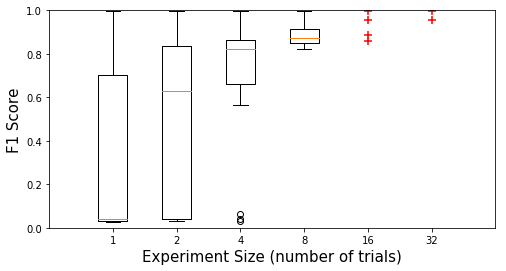
\includegraphics[width=0.8\linewidth]{images/random_hp_search_dnn_easy}
	\caption{Random hyperparameter search efficiency curves for the DNN using the simplified dataset.}
	\label{fig:random_hp_search_dnn_easy}
\end{figure}

\begin{figure}[H]
	\centering
	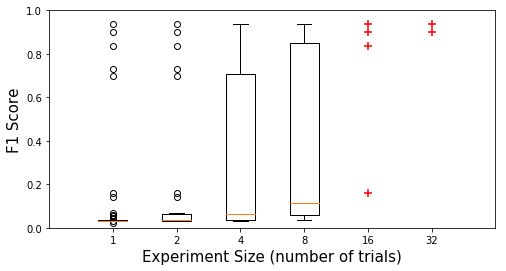
\includegraphics[width=0.8\linewidth]{images/random_hp_search_dnn_full}
	\caption{Random hyperparameter search efficiency curves for the DNN using the complete dataset.}
	\label{fig:random_hp_search_dnn_full}
\end{figure}


Figure \ref{fig:dense_hyperparameters_f1_score} shows the distribution of random hyperparameters and their average F1 score from the k-folds testing set. Sub-figure \ref{fig:learning_rate_learning} shows that a learning rate less than 10$^{-2}$ should be used for future hyperparameter searches. This figure also shows that the more difficult dataset prefers a slower learning rate. 


\begin{figure}[H]
     \centering
     \begin{subfigure}[b]{0.49\textwidth}
         \centering
         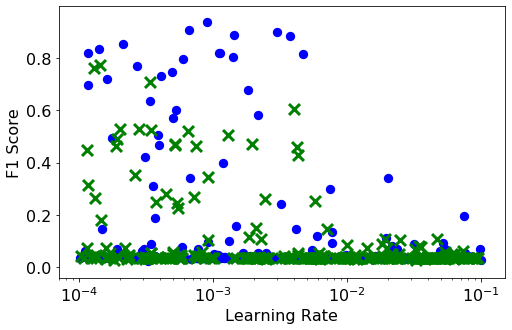
\includegraphics[width=\textwidth]{images/dnn_learning_rate.png}
         \caption{Learning Rate}
         \label{fig:dnn_learning_rate}
     \end{subfigure}
     \hfill
     \begin{subfigure}[b]{0.49\textwidth}
         \centering
         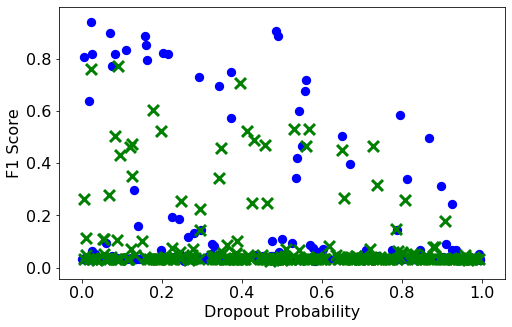
\includegraphics[width=\textwidth]{images/dnn_dropout.png}
         \caption{Dropout Rate}
         \label{fig:dnn_dropout}
     \end{subfigure}

     \begin{subfigure}[b]{0.49\textwidth}
         \centering
         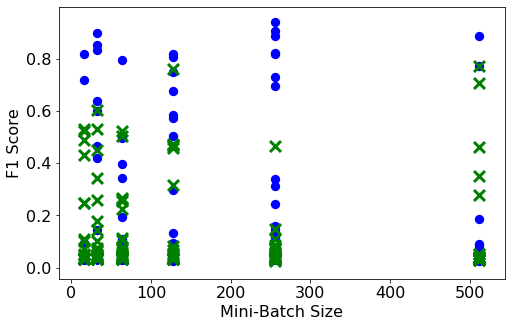
\includegraphics[width=\textwidth]{images/dnn_batch_size.png}
         \caption{Batch Size}
         \label{fig:dnn_batch_size}
     \end{subfigure}
     \hfill
     \begin{subfigure}[b]{0.49\textwidth}
         \centering
         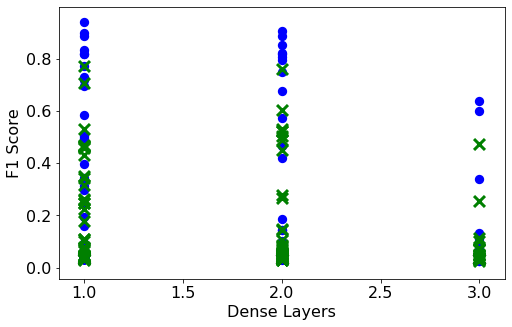
\includegraphics[width=\textwidth]{images/dnn_dense_layers_total.png}
         \caption{Total Dense Layers}
         \label{fig:dnn_dense_layers_total}
     \end{subfigure}

    \begin{subfigure}[b]{0.49\textwidth}
         \centering
         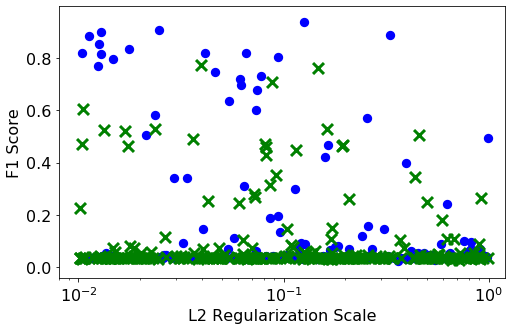
\includegraphics[width=\textwidth]{images/dnn_l2_reg.png}
         \caption{L2 Regularization Scale}
         \label{fig:dnn_l2_reg}
     \end{subfigure}
     \hfill
     \begin{subfigure}[b]{0.49\textwidth}
         \centering
         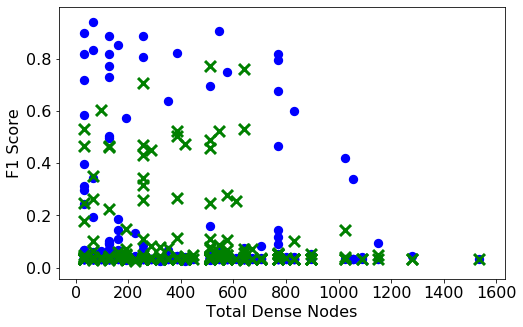
\includegraphics[width=\textwidth]{images/dnn_dense_nodes_total.png}
         \caption{Total Nodes}
         \label{fig:dnn_dense_nodes_total}
     \end{subfigure}     

     \begin{subfigure}[b]{0.49\textwidth}
         \centering
         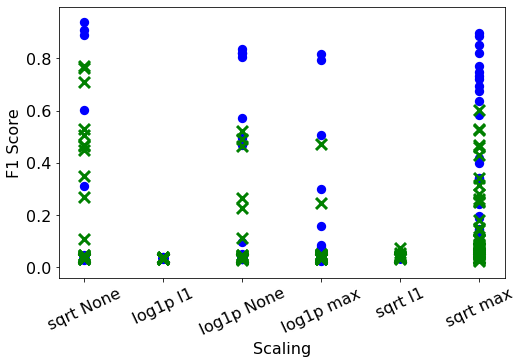
\includegraphics[width=\textwidth]{images/dnn_scaler.png}
         \caption{Feature Scaling}
         \label{fig:dnn_scaler}
     \end{subfigure}

        \caption{Effect of hyperparameters on F1 score. Blue circles represent the simple dataset, green crosses are the complete dataset.}
        \label{fig:dense_hyperparameters_f1_score}
\end{figure}


In addition to hyperparameters associated with the DNN's architecture and training, hyperparameters explored include the autoencoder used. Autoencoders can generate a different encoding based on a given architecture. The mean squared reconstruction error may not be the best metric to measure how good this encoding is as a preprocessing step. To determine an optimum preprocessing architecture for the dense and convolutional autoencoder, the choice of preprocessing architectures was added as a hyperparameter. The choices belong to the set with the N best reconstruction errors, respective of dense and convolution architecture.

% \subsubsection{Hyperparameter Search Results - Autoencoders}

% Now that we know optimized autoencoder architectures for the DNN, we need to optimize training hyperparameters. 

% https://machinelearningmastery.com/activation-regularization-for-reducing-generalization-error-in-deep-learning-neural-networks/

% \cite{Ranzato2007} Fig 6 shows you can freeze the unsupervised feature extraction network and update the classifier if you have enough data.

% Sparse denoising autoencoders are included in in this work as feature extraction and dimension reduction techniques. Both autoencoders employ regularization techniques to ensure useful representations are learned. Both models includes $l1$ activity regularization as a method to induce sparsity on the networks activations, which increases generalization \cite{Goodfellow-et-al-2016}. 

% Show how well autoencoders worked at spectrum reconstruction and background subtraction. See if there's a large difference between doing background subtraction and 


\subsection{Convolution Architecture}

Just like the autoencoder, this can be done in one or two steps. One step: Train and optimize the entire network, convolution and dense layers. Two steps: Train and optimize the dense layer, using random initialization for non-trainable convolution filters. We'll probably go with the two-step.

\begin{table}[H]
\centering
\caption{Range of hyperparameters explored for the CNN.}
\label{table:hyperparameter_dataset_parameters_CNN}
\begin{tabular}{ccc}
% \cline{2-3}
 & Hyperparameter Range & Sampling \\ \hline
\multicolumn{1}{c}{Number of Filter Kernels} & \begin{tabular}[c]{@{}c@{}}(4)   (8)   (16)    (32)\\ (4, 8)  (8, 16)  (16, 32)\\ (4, 8, 16)   (8, 16, 32)\end{tabular} & Uniform \\
\multicolumn{1}{c}{Filter Kernel Length} & 2, 4, 8, 16 & Uniform \\
\multicolumn{1}{c}{Pooling size} & 2, 4, 8, 16 & Uniform \\
\multicolumn{1}{c}{Number of Dense Layers} & 1 - 3 & Uniform \\
\multicolumn{1}{c}{Nodes in Dense Layers} & 10 - 1000 & Log-Uniform \\
\multicolumn{1}{c}{Initial Learning Rate} & 10$^{-4}$ - 10$^{-1}$ & Log-Uniform \\
\multicolumn{1}{c}{L2 Regularization Strength} & 10$^{-3}$ - 10$^{0}$ & Log-Uniform \\
\multicolumn{1}{c}{Dropout Frequency} & 0 - 1 & Uniform \\
\multicolumn{1}{c}{Batch Size} & 2$^{4}$ - 2$^{6}$ & Power of Two \\
\multicolumn{1}{c}{Activation Function} & tanh & Uniform \\
\multicolumn{1}{c}{Input Scaling} & \begin{tabular}[c]{@{}c@{}}sqrt, sqrt-max,\\sqrt-L1 Norm,\\ log1p-None, log1p-max,\\ log1p-L1 Norm\end{tabular} & Uniform \\
\end{tabular}
\end{table}


\begin{figure}[H]
	\centering
	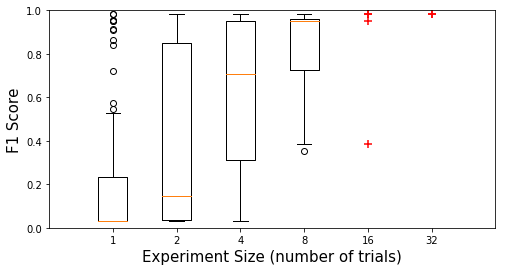
\includegraphics[width=0.8\linewidth]{images/random_hp_search_cnn_easy}
	\caption{Random hyperparameter search efficiency curves for the CNN using the simplified dataset.}
	\label{fig:random_hp_search_cnn_easy}
\end{figure}

\begin{figure}[H]
	\centering
	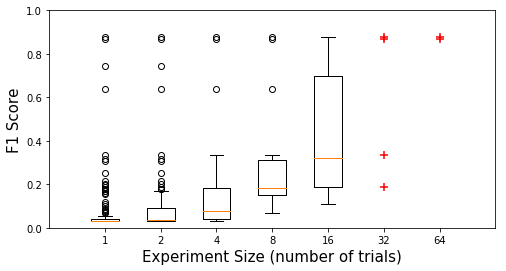
\includegraphics[width=0.8\linewidth]{images/random_hp_search_cnn_full}
	\caption{Random hyperparameter search efficiency curves for the CNN using the complete dataset.}
	\label{fig:random_hp_search_cnn_full}
\end{figure}





Figure \ref{fig:cnn_hyperparameters_f1_score} shows the distribution of random hyperparameters from the CNN and their average F1 score from the k-folds testing set. 


\begin{figure}[H]
     \centering
     \begin{subfigure}[b]{0.49\textwidth}
         \centering
         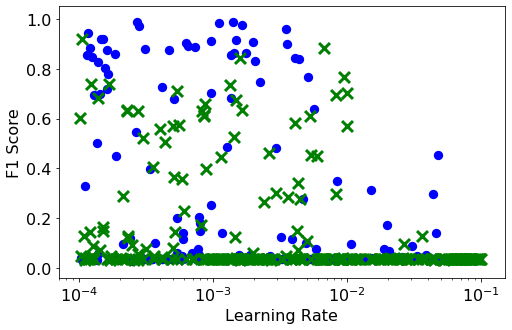
\includegraphics[width=\textwidth]{images/cnn_learning_rate.png}
         \caption{Learning Rate}
         \label{fig:cnn_learning_rate}
     \end{subfigure}
     \hfill
     \begin{subfigure}[b]{0.49\textwidth}
         \centering
         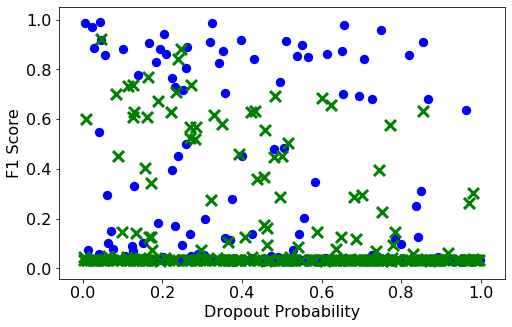
\includegraphics[width=\textwidth]{images/cnn_dropout.png}
         \caption{Dropout Rate}
         \label{fig:cnn_dropout}
     \end{subfigure}

     \begin{subfigure}[b]{0.49\textwidth}
         \centering
         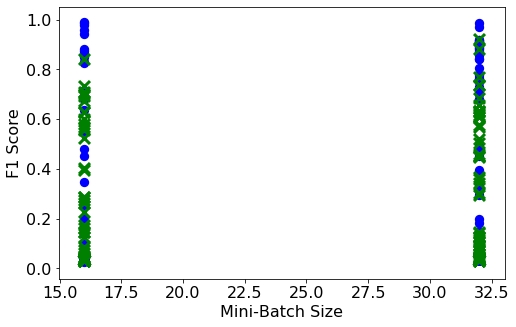
\includegraphics[width=\textwidth]{images/cnn_batch_size.png}
         \caption{Batch Size}
         \label{fig:cnn_batch_size}
     \end{subfigure}
     \hfill
     \begin{subfigure}[b]{0.49\textwidth}
         \centering
         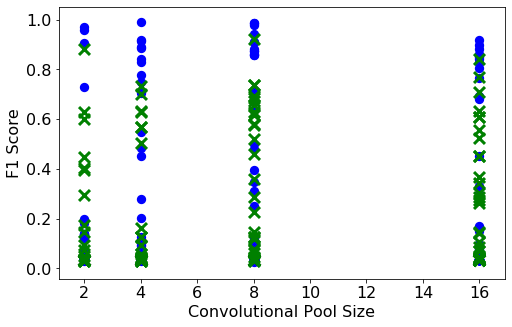
\includegraphics[width=\textwidth]{images/cnn_pooling_size.png}
         \caption{CNN Pooling Size}
         \label{fig:cnn_pooling_size}
     \end{subfigure}

    \begin{subfigure}[b]{0.49\textwidth}
         \centering
         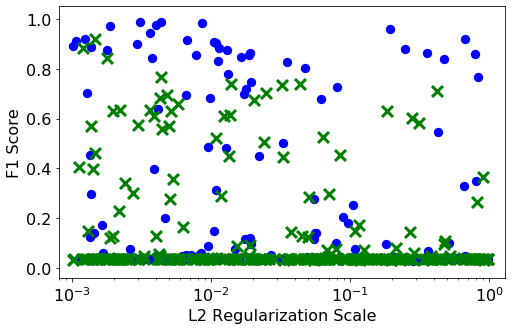
\includegraphics[width=\textwidth]{images/cnn_l2_reg.png}
         \caption{L2 Regularization Scale}
         \label{fig:cnn_l2_reg}
     \end{subfigure}
     \hfill
     \begin{subfigure}[b]{0.49\textwidth}
         \centering
         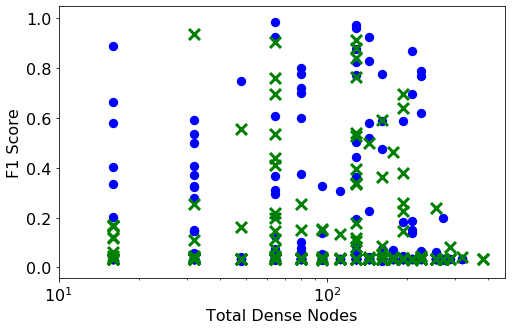
\includegraphics[width=\textwidth]{images/cnn_dense_nodes_total.png}
         \caption{Total Dense Nodes}
         \label{fig:cnn_dense_nodes_total}
     \end{subfigure}  
     
     \begin{subfigure}[b]{0.49\textwidth}
         \centering
         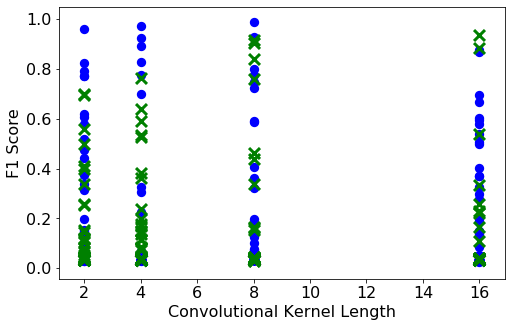
\includegraphics[width=\textwidth]{images/cnn_kernel_length.png}
         \caption{Convolution Kernel Length}
         \label{fig:cnn_kernel_length}
     \end{subfigure}
     \hfill
     \begin{subfigure}[b]{0.49\textwidth}
         \centering
         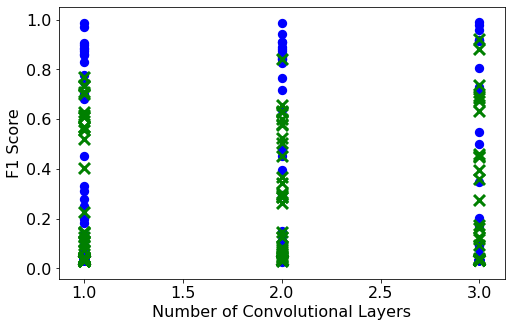
\includegraphics[width=\textwidth]{images/cnn_num_conv_layers.png}
         \caption{Total Convolution Layers}
         \label{fig:cnn_num_conv_layers}
     \end{subfigure}  
     
     \begin{subfigure}[b]{0.49\textwidth}
         \centering
         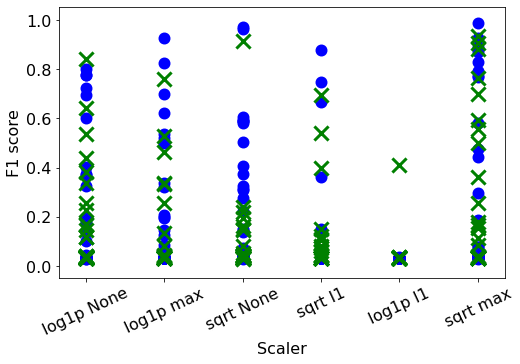
\includegraphics[width=\textwidth]{images/cnn_scaler.png}
         \caption{Feature Scaling}
         \label{fig:cnn_scaler}
     \end{subfigure}
     
        \caption{Effect of CNN hyperparameters on F1 score. Blue circles represent the simple dataset, green crosses are the complete dataset.}
        \label{fig:cnn_hyperparameters_f1_score}
\end{figure}


\section{Autoencoder Architectures}

Without an autoencoder, a single ANN has to learn multiple tasks to identify isotopes. An ANN would have to simultaneously identify the detector calibration, background signal, and source signal. By training an autoencoder to reconstruct a background-subtracted and correctly calibrated spectrum, the task of isotope identification is simplified for the ANN. This may result in more accurate identifications. 




To test this, for each dataset a single autoencoder and three ANNs will be trained. The first will be trained without an autoencoder. The second will be trained using the encoder as input. A random hyperparameter search will be used to find an appropriately structured autoencoder. The testing and validation error for these ANNs will be compared for each respective dataset.

\subsection{Autoencoder Structure Hyperparameter Search}

This section will explain the hyperparameter structures searched. The autoencoder used is a undercomplete denoising autoencoder \cite{Goodfellow-et-al-2016}. Because the denoising operation performs regularization implicitly, no additional regularization is added to the autoencoders. 

The autoencoder structures are found using a grid search. The autoencoders that reproduce the background subtracted signal the best are used in a dense random hyperparameter search as the signal preprocessing.


\subsubsection{Dense Autoencoder Structure}


\begin{table}[H]
\centering
\caption{Hyperparameters used in the grid search for the DAE architecture.}
\label{table:hyperparameters_DAE}
\begin{tabular}{ccc}
% \cline{2-3}
 & Hyperparameter Range & Sampling \\ \hline
\multicolumn{1}{c}{Architectures} & \begin{tabular}[c]{@{}c@{}}sqrt, sqrt-max,\\ sqrt-L1 norm,\\ log1p, log1p-max,\\ log1p-L1 norm\end{tabular} & Uniform \\
\multicolumn{1}{c}{Initial Learning Rate} & 10$^{-3}$ & N/A \\ 
\multicolumn{1}{c}{Batch Size} & 32 & N/A \\ 
\multicolumn{1}{c}{Activation Function} & relu, tanh & Uniform \\ 
\multicolumn{1}{c}{Input Scaling} & \begin{tabular}[c]{@{}c@{}}sqrt, sqrt-max,\\ sqrt-L1 norm,\\ log1p, log1p-max,\\ log1p-L1 norm\end{tabular} & Uniform \\
\end{tabular}
\end{table}

\subsubsection{Convolutional Autoencoder Structure}

\begin{table}[H]
\centering
\caption{Hyperparameters used in the grid search for the CAE architecture.}
\label{table:hyperparameters_CAE}
\begin{tabular}{ccc}
% \cline{2-3}
 & Hyperparameter Range & Sampling \\ \hline
\multicolumn{1}{c}{Architectures} & \begin{tabular}[c]{@{}c@{}}sqrt, sqrt-max,\\ sqrt-L1 norm,\\ log1p, log1p-max,\\ log1p-L1 norm\end{tabular} & Uniform \\
\multicolumn{1}{c}{Initial Learning Rate} & 10$^{-3}$ & N/A \\ 
\multicolumn{1}{c}{Batch Size} & 32 & N/A \\ 
\multicolumn{1}{c}{Activation Function} & relu, tanh & Uniform \\ 
\multicolumn{1}{c}{Input Scaling} & \begin{tabular}[c]{@{}c@{}}sqrt, sqrt-max,\\ sqrt-L1 norm,\\ log1p, log1p-max,\\ log1p-L1 norm\end{tabular} & Uniform \\
\end{tabular}
\end{table}



\subsection{Autoencoder Performance}

In this section, we perform a random hyperparameter search for dense networks using the autoencoders. 


\begin{table}[H]
\centering
\caption{Range of hyperparameters explored for the dense network.}
\label{table:hyperparameter_dataset_parameters_DAE}
\begin{tabular}{ccc}
% \cline{2-3}
 & Hyperparameter Range & Sampling \\ \hline
\multicolumn{1}{c}{Number of Layers} & 1 - 3 & Uniform \\ 
\multicolumn{1}{c}{Nodes in Layer} & 2$^{5}$ - 2$^{10}$ & Power of Two \\ 
\multicolumn{1}{c}{Initial Learning Rate} & 10$^{-4}$ - 10$^{-1}$ & Logarithmic \\ 
\multicolumn{1}{c}{L2 Regularization Strength} & 10$^{-2}$ - 10$^{0}$ & Logarithmic \\ 
\multicolumn{1}{c}{Dropout Frequency} & 0 - 1 & Uniform \\ 
\multicolumn{1}{c}{Batch Size} & 2$^{4}$ - 2$^{10}$ & Power of Two \\ 
\multicolumn{1}{c}{Activation Function} & relu, tanh & Uniform \\ 
\multicolumn{1}{c}{Input Scaling} & \begin{tabular}[c]{@{}c@{}} sqrt-DAE, log1p-DAE,\\sqrt-L1 Norm,\\ log1p-None, log1p-max,\\ log1p-L1 Norm\end{tabular} & Uniform \\
\end{tabular}
\end{table}











\begin{table}[H]
\centering
\caption{Comparison of fixed and pretrained autoencoders.}
\label{table:autoencoders_fixed_pretrained}
\begin{tabular}{cc}
Model & Test Set F1 Score \\  \hline
\begin{tabular}[c]{@{}c@{}}CAE-DNN\\ fixed\end{tabular} & 0.4 \\ 
\begin{tabular}[c]{@{}c@{}}CAE-DNN as\\ pretraining\end{tabular} & 0.4 \\ 
\begin{tabular}[c]{@{}c@{}}DAE-DNN\\ fixed\end{tabular} & 0.4 \\ 
\begin{tabular}[c]{@{}c@{}}DAE-DNN as\\ pretraining\end{tabular} & 0.4 \\ 
\end{tabular}
\end{table}




\begin{figure}[H]
	\centering
	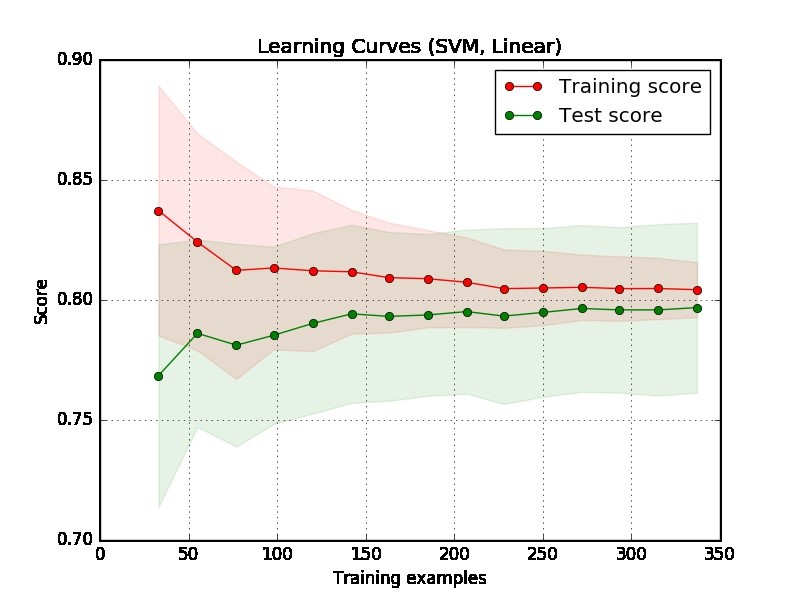
\includegraphics[width=0.8\linewidth]{model_choice_hyperparameter_search_images/learning_curve_dummy}
	\caption{Training curves for the fixed and pretraining DAE-DNN's, CAE-DNN's.}
	\label{fig:learning_curves}
\end{figure}




\section{Summary of Final Model Architectures}


This section discusses performance differences between the DNN, CNN, CAE-DNN, and DAE-DNN. These differences will be based on the final testing set error for all models.  





